\section{Ejercicio 2}

% Para convencer a Marty, el Doc necesita mostrarle un algoritmo que
% efectivamente resuelva el problema. Dado que sus habilidades de programador
% están un poco oxidadas, se les pide diseñar e implementar un algoritmo
% exacto para MCS y desarrollar los siguientes puntos que justifiquen la
% solución encontrada:
% a) Explicar detalladamente el algoritmo implementado. Elaborar podas y
%    estrategias que permitan mejorar los tiempos de resolución.
% b) Calcular el orden de complejidad temporal de peor caso del algoritmo.
% c) Realizar una experimentación que permita observar los tiempos de
%    ejecución del algoritmo en función del tamaño de entrada y de las podas
%    y/o estrategias implementadas.

\subsection{Introducción}
En este ejercicio, se busca encontrar un algoritmo exacto para resolver, en
tiempo exponencial, el problema del \acr{MCS} entre dos grafos cualquiera.
Para ello utilizamos el método de \textit{Backtracking}. Este método es
extremadamete costoso tanto temporal como espacialmente, por lo que no sólo
es recomendable sino condición del ejercicio realizar podas y estrategias que
permitan mejorar los tiempos de resolución.

\subsection{Resolución}
El algoritmo consiste en probar todos los mapeos posibles entre los nodos de
ambos grafos, y así tomar un grafo común con la mayor cantidad de aristas de
entre todas las combinaciones de mapeos.

Dentro de la función principal, aquella que emplea la técnica de
\textit{Backtracking}, se hace uso de ambos grafos, otro grafo que representa
el subgrafo común máximo dentro de la rama de ejecución (inicialmente
vacío), dos listas enlazadas (una para cada grafo) que contienen
los ids de los nodos aún no mapeados en esta rama de ejecución, y un mapa
implementado sobre una tabla de hash que contiene los mapeos hechos en esa
rama de ejecución.

~

\begin{algorithm}[H]
    \caption{MCSBacktracking}
    \label{algo:backtracking}

    \Input{Dos grafos $g_1$ y $g_2$ donde los nodos se representan con enteros,
    el subgrafo común máximo de esta rama de ejecución $mcs$ pasado por
    referencia (cada nodo en este subgrafo consiste de un par de enteros que
    representa el mapeo entre nodos de $g_1$ y $g_2$, dos listas enlazadas
    $l_1$ y $l_2$ y un mapa $mapeos$.}
    \Output{Un booleano que indica si el subgrafo pasado por referencia es
    válido (para más adelante efectuar podas).}

    \If {$l_1$.vacia() $\lor$ $l_2$.vacia()} {
        \Return{verdadero}
    }

    $maxMCS$ $\gets$ grafo de pares vacío \;

    \For {$nodo_1 \in l_1$} {
        \For {$nodo_2 \in l_2$} {

            $l_1$.borrar($nodo_1$) \;
            $l_2$.borrar($nodo_2$) \;

            $copiaMapeos$ $\gets$ $mapeos$ \;
            $copiaMapeos$.insertar($nodo_1$, $nodo_2$) \;

            $copiaMCS$ = $mcs$.clonar() \;
            $copiaMCS$.agregarNodo(par($nodo_1$, $nodo_2$)) \;

            \For {$vecino \in g_1$.vecinos($nodo_1$)} {
                $mapeadoAVecino$ $\gets$ $mapeos$.valor($vecino$) \;
                \If {$mapeos$.esta($vecino$) $\land g_2$.adyacentes($nodo_2$,
                $mapeadoAVecino$) } {
                    $copiaMCS$.agregarEje(par($nodo_1$, $nodo_2$), par($vecino$,
                    $mapeadoAVecino$))
                }
            }

            MCSBacktracking($g1$, $g2$, $copiaMCS$, $copiaMapeos$, $l_1$, $l_2$) \;

            \If {$MCSBacktraking$ es valido $\land copiaMCS$.m() $\geq maxMCS$.m()} {
                $maxMCS$ $\gets$ $copiaMCS$ \;
            }

            $l_1$.reinsertar($nodo_1$) \;
            $l_2$.reinsertar($nodo_2$) \;
        }
    }

    $mcs$ $\gets$ $maxMCS$

    \Return{veradero}
\end{algorithm}

Lo que se expone en el algoritmo \ref{algo:backtracking} es el pseudocódigo
del algoritmo principal. Por simplicidad, evitaremos las podas del algoritmo
momentaneamente. Posteriormente ahondaremos en ellas.

Se iteran $l_1$ y $l_2$
mediante dos ciclos anidados para de esta forma probar todos los elementos de
$l_1$ contra todos los de $l_2$ formando todos los pares de nodos posibles.
Dentro de la doble iteración se prueba el mapeo de los dos nodos seleccionados
actualizando las listas de nodos restantes y el mapa, y se hace el llamado
recursivo pasando una copia del \textit{mcs} por referencia, al cual se le
añade previamente un nodo que representa el mapeo.

Una vez terminados los ciclos se le asigna la mayor de las copias de
\textit{mcs} al subgrafo pasado por referencia.

\subsubsection{Podas y optimizaciones}

Se puede apreciar en el pseudocódigo anterior la existencia de una condición
para asignar el \textit{mcs} obtenido a la variable que almacena el máximo de
las iteraciones tras el llamado recursivo (aparte de la que verifica si es
mayor en cantidad de aristas). Se pide que el resultado del llamado haya sido
válido, que es lo mismo que pedir que el valor retornado por la misma sea
verdadero. Esto pareciera no tener sentido, ya que en todos los casos el valor
devuelto es verdadero, pero eso es porque no están incluídas las podas. La
forma de podar el árbol de ejución que utilizamos hace uso de esa condición,
si se decide cortar la rama de ejecución entonces se devuelve falso y esta
estructura evitará chequeos innecesarios.

Las podas implementadas fueron las siguentes:

\begin{enumerate}
\item Verificar que la suma de los grados de los nodos que aun no han sido
mapeados pueda ser mayor que la máxima cantidad de aristas alcanzada hasta
el momento. De no ser así, se detiene y se corta la rama que está siendo
explorada.
\item Evitar armar grafos donde las permutaciones de mapeos representan el
mismo grafo.
\end{enumerate}

La verificación de la suma de los grados es sencilla. Consta de recorrer la
lista de nodos restantes e ir sumando los grados de cada uno de ellos. Si esa
suma junto con la cantidad de ejes del \textit{mcs} actual no puede superar
a la cantidad de ejes del máximos \textit{mcs} alcanzado en alguna de las
ramas de la ejecución previamente visitadas, entonces no tiene caso seguir
porque no es posible llegar a una mejor solución, por lo que se corta la
ejecución.

Para esto se hace uso de una estructura condicional que termina el llamado
devolviendo falso. Esta estructura es lo primero que se ejecuta cuando se hace
el llamado recursivo. Veamos un pseudocódigo.

\begin{algorithm}
    \caption{Poda de suma de grados}
    \If {$mcs$.m() + sumaDeGrados($l_1$) $\leq$ $maximaCantEjes$} {
        \Return{falso}
    }
\end{algorithm}

$maximaCantEjes$ es una referencia a una variable que es pasada por parámetro
en el llamado recursivo y que se acutaliza si se encuentra un mejor
\textit{mcs}.

La otra poda se enfoca en evitar inspeccionar una solución cuya rama de
ejecución es equivalente a una visitada anteriormente. Por ejemplo, tomemos
los grafos $A$ y $B$ con nodos $a_1, ..., a_n$ y $b_1, ..., b_k$. Durante la
ejecución del algoritmo se mapearán todas las posibles combinaciones entre
los nodos de estos grafos. Al mapearlos hay un orden que intríncecamente
determina cual es el mejor grafo en común, es decir, según que par de nodos
se mapeen, en el siguiente llamado recursivo el mapeo de otros dos nodos
será más eficiente o no en cuestión de cantidad de aristas del \textit{mcs}.
Pero aún así, cuando el conjunto de pares de nodos mapeados es el mismo (esto
aplica para cualquier momento del algoritmo, no necesariamente tienen que
haber sido mapeados todos los nodos) puede ser permutado y el \textit{mcs}
entre los grafos será el mismo, puesto que los nodos elegidos son los mismos.
Por esto es que la intención de esta poda es evitar llegar a un grafo con el
mismo conjunto de nodos mapeados, para así ahorrar llamados.

A continuación puede verse la imagen de un ejemplo de dos grafos junto con el
árbol de mapeos que se formailustrando la idea.

\begin{center}
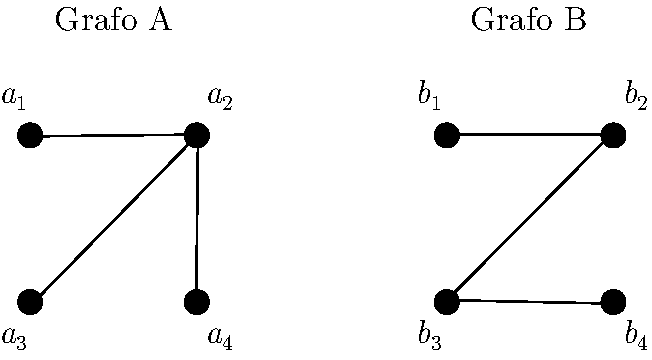
\includegraphics[width=.45\textwidth]{imagenes/ex2_grafos.pdf}
\end{center}

Las ramas en rojo son equivalentes, es decir, que representan la formación de
subgrafos comunes máximos isomorfos.

\begin{center}
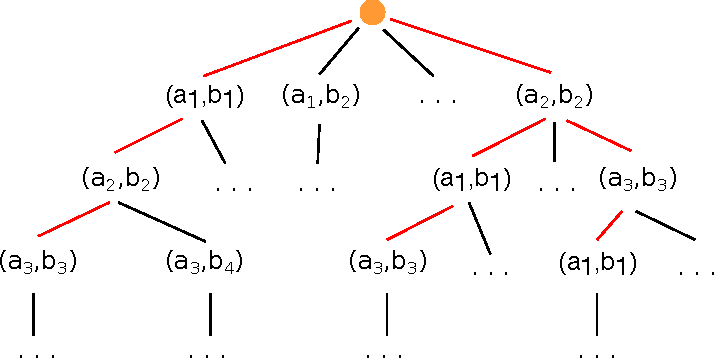
\includegraphics[width=.7\textwidth]{imagenes/ex2_execution_tree.pdf}
\end{center}

Para lograr esto utilizamos una referencia a una variable que es pasada por
parametro en el llamado recursivo que almacena conjuntos de pares. La idea es
que antes de hacer un llamado recursivo se busque dentro de este conjunto
si mi actual conjunto de mapeos ya ha sido visitado. De ser así entonces no se
hace el llamado sino que continúa la iteración formando un nuevo par para ser
mapeado en lugar del que ha sido rechazado.

El problema con esta idea es que tiene un costo temporal demasiado alto, al
punto de representar una desventaja, ya que la comparación entre dos conjuntos
implica gran cantidad de operaciones, y esto hay que hacerlo con todos los
conjuntos de pares del mismo cardinal. A medida que la cantidad de nodos
mapeados aumenta, se vuelve más costoso, y a su vez, menos provechoso debido
a que al llegar a un nivel más profundo en la rama de ejecución, la cantidad
de llamados que pueden ser omitidos es menor.

De modo que decidimos hacer efectiva esta poda únicamente para el segundo
nivel del árbol de ejecución. De esta forma las estructuras posibles se
simplificarían lo suficiente como para requerir una baja complejidad temporal.
Y además es el nivel en el que mas ramas se pueden descartarse.

La implementación de esta poda se realiza dentro del ciclo anidado, justo
después de haber elegido los nodos candidatos a ser mapeados. Veamos un
pseudocódigo.

\begin{algorithm}
    \caption{Poda permutaciones}
    \If {$mcs$.n() == 1} {
        $permutacion$ $\gets$ tupla con el primer par mapeado y el par actual \;
        \If {$permutaciones$.esta($permutacion$)} {
            romper el ciclo \;
        }
        \Else {
            $permutaciones$.guardar($permutacion$) \;
        }
    }
\end{algorithm}

$permutaciones$ es un conjunto implementado sobre un conjunto de hash.

La cantidad de hojas del árbol de ejecución que se ahorran es igual al
producto entre la cantidad de mapeos posibles en cada nivel, desde el tercero
hasta el último. La cantidad de mapeos posibles en un nivel es igual al
producto entre la cantidad de nodos restantes de cada grafo. Entonces la
cantidad de hojas ahorradas es igual a $(n_1 - 2) \times (n_2 - 2) \times
(n_1 - 3) \times (n_2 - 3) \times ... \times 1 \times (n_2 - n_1 + 1)$ si
suponemos que el segundo grafo es mayor o igual que el primero. Esto es
equivalente a $\frac{(n_1 - 2)! \times (n_2 - 2)!}{(n_2 - n_1)!}$, por lo que
fácilmente puede apreciarse por qué esta poda resultaría buena.

En un principio pensábamos que estas podas no resultarían demasiado efectivas,
e incluso dudábamos si el costo de cada una no pudiese significar una
desmejora en relación a la ganancia. Nos equivocamos. Ambas podas no sólo
acabaron siendo muy buenas, sino fundamentales a medida que el tamaño de los
grafos crecía.

\subsection{Complejidad}

Para medir la complejidad del algoritmo, en principio, se analizará el
árbol de ejecución dado por el mismo. Se definen $n_1$ y $n_2$ las cantidades
de nodos de los grafos, y se supone $n_1 \leq n_2$. Por cada llamado de
la función, se hace una cantidad de llamados recursivos que depende de en qué
nivel del árbol de ejecución se encuentre actualmente el algoritmo. Esto es
así debido a que el llamado recursivo se encuentra dentro del ciclo anidado,
y la cantidad de iteraciones de ese ciclo depende de la cantidad de nodos que
aún no han sido mapeados. Como en cada llamado se mapea un par de nodos, la
cantidad de nodos por mapear va disminuyendo en cada nivel.

Para el nivel $i$ la cantidad de veces que se hace el llamado es de
$(n_1 - i)  (n_2 - i)$, que es resultado de probar todos los posibles
pares entre los nodos restantes de ambos grafos. De esta forma, la cantidad de
llamados en un nivel es de
$\frac{n_1!  n_2!}{(n_1 - i)!  (n_2 - i)!}$.

Ahora se hará enfoque en la complejidad del algoritmo en para cada nivel $i$.

\begin{itemize}
\item Se recorren linealmente los nodos restantes para saber si es posible
efectuar la poda de la suma de grados. $\ord(n_1 - i)$.
\item Dentro del doble ciclo anidado que se ejecuta
$(n_1 - i)  (n_2 - i)$ veces
\begin{itemize}
\item Copiar el mapa. $\ord(i)$.
\item Clonar subgrafo. $\ord(i)$
\item Agregar nodo. $\ord(i)$
\item Agregar ejes al nuevo nodo del \textit{mcs}. Lineal sobre la cantidad de
vecinos del nuevo nodo.
\item Mover iteradores hasta la posicion correspondiente.
$\ord(n_1 - i + n_2 - i)$
\end{itemize}
Entones el doble ciclo tiene complejidad

$\sum_{k = 1}^{n_1 - i} \sum_{j = 1}^{n_2 - i} (\ord(i) + \ord(deg(v_{kj}) +$
$ \ord(n_1 + n_2 - 2i))=$

$\sum_{k = 1}^{n_1 - i} \sum_{j = 1}^{n_2 - i} (\ord(deg(v_{kj}) +$
$ \ord(n_1 + n_2))=$

$\ord((n_1 - i)  (n_2 - i)  (n_1 + n_2)) + \sum_{k = 1}^{n_1 - i}$
$ \sum_{j = 1}^{n_2 - i} \ord(deg(v_{kj}))$.

Puede acotarse superiormente el grado de $v_{kj}$ por $n_1$ ya que no puede
tener más de $n_1 - 1$ vecinos. Entonces la complejidad es

$\ord((n_1 - i)  (n_2 - i)  (n_1 + n_2)) + \sum_{k = 1}^{n_1 - i}$
$\sum_{j = 1}^{n_2 - i} \ord(n_1)=$

$\ord((n_1 - i)  (n_2 - i)  (n_1 + n_2)) + \ord((n_1 - i) $
$(n_2 - i)  n_1)=$

$\ord((n_1 - i)  (n_2 - i)  (n_1 + n_2 + n_1))=$

$\ord((n_1 - i)  (n_2 - i)  (n_1 + n_2))$.
\end{itemize}

Por lo tanto la complejidad en cada nivel $i$ es $\ord(n_1 - i) +$
$\ord((n_1 - i)  (n_2 - i)  (n_1 + n_2)) = \ord((n_1 - i) $
$ (n_2 - i)  (n_1 + n_2))$.

La cantidad de niveles que tiene el árbol de ejecución es de $n_1$ ya que se
hacen llamados recursivos hasta que uno de los grafos tenga todos sus nodos
mapeados. Como ya vimos en cada nivel se hacen
$\frac{n_1!  n_2!}{(n_1 - i)!  (n_2 - i)!}$ llamados, por lo que
la cantidad total de llamados es de
$\sum_{i = 0}^{n_1} \frac{n_1!  n_2!}{(n_1 - i)!  (n_2 - i)!}$.

Puede acotarse esta cantidad de llamados superiormente de modo que sea
$\ord(n_1  \frac{n_1!  n_2!}{(n_2 - n_1)!})$ siendo $n_1$ la
cantidad de niveles y $\frac{n_1!  n_2!}{(n_2 - n_1)!}$ la de hojas.

~

Entonces la complejidad total del algoritmo es

$\sum_{i = 0}^{n_1}[\frac{n_1!  n_2!}{(n_1 - i)!  (n_2 - i)!}$
$ \ord((n_1 - i)  (n_2 - i)  (n_1 + n_2))]=$
$\ord(n_1  \frac{n_1!  n_2!}{(n_2 - n_1)!}) $
$\sum_{i = 0}^{n_1}\ord((n_1 - i)  (n_2 - i)$
$ (n_1 + n_2))$.

~

Desarrollando
$\sum_{i = 0}^{n_1}\ord((n_1 - i)  (n_2 - i)$
$ (n_1 + n_2))=$
$(n_1 + n_2)  \sum_{i = 0}^{n_1}\ord((n_1 - i)  (n_2 - i))$

~

Sea $j = n_1 - i$ y por consecuente $i = n_1 - j$ se verifica que

$\ord((n_1 + n_2))  \sum_{i = 0}^{n_1} \ord((n_1 - i)  (n_2 - i))=$

$\ord((n_1 + n_2))  \sum_{j = 0}^{n_1} (\ord(j)  (n_2 - n_1 + j))=$

$\ord((n_1 + n_2))  \sum_{j = 0}^{n_1} (\ord(j^2) + j  (n_2 - n_1))=$

$\ord((n_1 + n_2))  \ord(\sum_{j = 0}^{n_1} j^2) + (n_2 - n_1)  \sum_{j = 0}^{n_1} j)=$

$\ord((n_1 + n_2))  \ord(\frac{1}{6}n_1(n_1 + 1)(2n_1 + 1) + \frac{1}{2}(n_2 - n_1)n_1(n_1 + 1))=$

$\ord((n_1 + n_2))  \ord(\frac{1}{6}(2n_1^3 + 3n_1^2 + n_1) + \frac{1}{2}(n_2 - n_1)(n_1^2 + n_1))=$

$\ord((n_1 + n_2))  \ord(\frac{1}{6}(2n_1^3 + 3n_1^2 + n_1) + \frac{1}{2}(n_1^2n_2 - n_1^3 + n_1n_2 - n_1^2))=$

$\ord((n_1 + n_2))  \ord(\frac{1}{6}(2n_1^3 + 3n_1^2 + n_1) + \frac{1}{6}(3n_1^2n_2 - 3n_1^3 + 3n_1n_2 - 3n_1^2))=$

$\ord((n_1 + n_2))  \ord(\frac{1}{6}(2n_1^3 + 3n_1^2 + n_1 + 3n_1^2n_2 - 3n_1^3 + 3n_1n_2 - 3n_1^2))=$

$\ord((n_1 + n_2))  \ord(\frac{1}{6}(-n_1^3 + n_1 + 3n_1^2n_2 + 3n_1n_2))=$

$\ord((n_1 + n_2))  \ord(\frac{1}{6}n_1(-n_1^2 + 1 + 3n_1n_2 + 3n_2))=$

$\ord((n_1 + n_2))  \ord(n_1^2n_2)=$

$\ord((n_1 + n_2)  n_2  n_1^2)$

~

Finalmente, la complejidad del algoritmo es
$\ord(n_1  \frac{n_1!  n_2!}{(n_2 - n_1)!}) \ord((n_1 + n_2)  n_2  n_1^2)=$

\begin{center}
$\ord(\frac{n_1!  n_2!}{(n_2 - n_1)!} (n_1 + n_2)  n_2  n_1^3)$
\end{center}

\subsection{Experimentación}

Como fue visto anteriormente, la complejidad del algoritmo es
$\ord(\frac{n_1!  n_2!}{(n_2 - n_1)!} (n_1 + n_2)  n_2  n_1^3)$ siempre que
valga $n_1 \leq n_2$.

Cubrir un amplio espectro.

Para evitar la interferencia en las mediciones de la morfología del grafo, se
fijó cada experimento para una familia de grafos determinada. Así, se tiene un
mayor control de las variables involucradas. Sin embargo, para verificar que
la cota teórica de complejidad no se cumple de forma accidental, sino que vale
para grafos de cualquier tipo, se probó con varias familias distintas.

\begin{figure}[H]
    \label{fig:exp2:n_1=n_2}
    \centering
    \begin{tikzpicture}
        \begin{axis}[
                title={},
                xlabel={Cantidad de nodos ($n_1$)},
                ylabel={Tiempo de ejecución (nanosegundos)},
                scaled x ticks=false,
                scaled y ticks=false,
                enlargelimits=0.05,
                width=0.5\textwidth,
                height=0.5\textwidth,
                legend pos=north west,
                legend cell align=left,
                ymode=log
                % xmin=100
            ]
            \addplot[color=black] table[x index=0,y index=1]{../exp/ej2/equal_complete_vs_complete};
            \addplot[color=blue] table[x index=0,y index=1]{../exp/ej2/equal_tree_vs_tree};

            \legend{$T_{(co_n)}$}
        \end{axis}
    \end{tikzpicture}
    \caption{Tiempos de ejecución observados para $n_1 = n_2$.}
\end{figure}